\documentclass[12pt, titlepage]{article}

\usepackage{fullpage}
\usepackage[round]{natbib}
\usepackage{multirow}
\usepackage{booktabs}
\usepackage{tabularx}
\usepackage{graphicx}
\usepackage{float}
\usepackage{hyperref}
\hypersetup{
    colorlinks,
    citecolor=black,
    filecolor=black,
    linkcolor=red,
    urlcolor=blue
}
\usepackage[round]{natbib}
\usepackage{color}
\usepackage{xcolor}

\newcounter{acnum}
\newcommand{\actheacnum}{AC\theacnum}
\newcommand{\acref}[1]{AC\ref{#1}}

\newcounter{ucnum}
\newcommand{\uctheucnum}{UC\theucnum}
\newcommand{\uref}[1]{UC\ref{#1}}

\newcounter{mnum}
\newcommand{\mthemnum}{M\themnum}
\newcommand{\mref}[1]{M\ref{#1}}

\title{SE 3XA3: Software Requirements Specification\\
  Finite State Machine Simulator}

\author{Team \#16, NonDeterministic Key
		\\ Anhao Jiao (jiaoa3)
		\\ Kehao Huang (huangk53)
		\\ Xunzhou Ye (yex33)
}

\date{18 March 2022}



\begin{document}

\maketitle

\pagenumbering{roman}
\tableofcontents
\listoftables
\listoffigures

\begin{table}[H]
  \caption{\bf Revision History}
  \begin{tabularx}{\textwidth}{p{3cm}p{2cm}X}
    \toprule {\bf Date} & {\bf Version} & {\bf Notes}\\
    \midrule
    March 18 & 0.1 & Partial complete MG \\
    \textcolor{red}{April 12} & \textcolor{red}{1.0} & \textcolor{red}{added use
                                                       hierarchy} \\
    \bottomrule
  \end{tabularx}
\end{table}

\newpage

\pagenumbering{arabic}

\section{Introduction}

Decomposing a system into modules is a commonly accepted approach to developing
software.  A module is a work assignment for a programmer or programming
team.  We advocate a decomposition
based on the principle of information hiding.  This
principle supports design for change, because the ``secrets'' that each module
hides represent likely future changes.  Design for change is valuable in SC,
where modifications are frequent, especially during initial development as the
solution space is explored.  

Our design follows the rules layed out by , as follows:
\begin{itemize}
\item System details that are likely to change independently should be the
  secrets of separate modules.
\item Each data structure is used in only one module.
\item Any other program that requires information stored in a module's data
  structures must obtain it by calling access programs belonging to that module.
\end{itemize}

After completing the first stage of the design, the Software Requirements
Specification (SRS), the Module Guide (MG) is developed. The MG
specifies the modular structure of the system and is intended to allow both
designers and maintainers to easily identify the parts of the software.  The
potential readers of this document are as follows:

\begin{itemize}
\item New project members: This document can be a guide for a new project member
  to easily understand the overall structure and quickly find the
  relevant modules they are searching for.
\item Maintainers: The hierarchical structure of the module guide improves the
  maintainers' understanding when they need to make changes to the system. It is
  important for a maintainer to update the relevant sections of the document
  after changes have been made.
\item Designers: Once the module guide has been written, it can be used to
  check for consistency, feasibility and flexibility. Designers can verify the
  system in various ways, such as consistency among modules, feasibility of the
  decomposition, and flexibility of the design.
\end{itemize}

The rest of the document is organized as follows. Section
\ref{SecChange} lists the anticipated and unlikely changes of the software
requirements. Section \ref{SecMH} summarizes the module decomposition that
was constructed according to the likely changes. Section \ref{SecConnection}
specifies the connections between the software requirements and the
modules. Section \ref{SecMD} gives a detailed description of the
modules. Section \ref{SecTM} includes two traceability matrices. One checks
the completeness of the design against the requirements provided in the SRS. The
other shows the relation between anticipated changes and the modules. Section
\ref{SecUse} describes the use relation between modules.

\section{Anticipated and Unlikely Changes} \label{SecChange}

This section lists possible changes to the system. According to the likeliness
of the change, the possible changes are classified into two
categories. Anticipated changes are listed in Section \ref{SecAchange}, and
unlikely changes are listed in Section \ref{SecUchange}.

\subsection{Anticipated Changes} \label{SecAchange}

\begin{description}
\item[\refstepcounter{acnum} \actheacnum :] The specific operating system on which the software is running.
\item[\refstepcounter{acnum} \actheacnum :] The format of the input data.
\item[\refstepcounter{acnum} \actheacnum :] The format of the output data.
\item[\refstepcounter{acnum} \actheacnum :] The instruction on how to use the software.
\end{description}

\subsection{Unlikely Changes} \label{SecUchange}

\begin{description}
\item[\refstepcounter{ucnum} \uctheucnum :] Input/Output devices
  (Input: Keyboard, Output: Picture, and Screen).
\item[\refstepcounter{ucnum} \uctheucnum :] The purpose of the software to generate \LaTeX\ snippets.
\end{description}

\section{Module Hierarchy} \label{SecMH}

This section provides an overview of the module design. Modules are summarized
in a hierarchy decomposed by secrets in Table \ref{TblMH}. The modules listed
below, which are leaves in the hierarchy tree, are the modules that will
actually be implemented.

\begin{description}
\item [\refstepcounter{mnum} \mthemnum \label{mHH}:] Hardware-Hiding Module
\item [\refstepcounter{mnum} \mthemnum \label{mMachine}:] Machine Module
\item [\refstepcounter{mnum} \mthemnum \label{mUtil}:] Util Module
\item [\refstepcounter{mnum} \mthemnum \label{mState}:] State Module
\item [\refstepcounter{mnum} \mthemnum \label{mCondition}:] Condition Module
\item [\refstepcounter{mnum} \mthemnum \label{mTransition}:] Transition Module
\item [\refstepcounter{mnum} \mthemnum \label{mEventData}:] EventData Module
\item [\refstepcounter{mnum} \mthemnum \label{mEvent}:] Event Module
\end{description}


\begin{table}[H]
\centering
\begin{tabular}{p{0.3\textwidth} p{0.6\textwidth}}
\toprule
\textbf{Level 1} & \textbf{Level 2}\\
\midrule

{Hardware-Hiding Module} & ~ \\
\midrule

\multirow{1}{0.3\textwidth}{Behaviour-Hiding Module} & Machine Module\\
\midrule

\multirow{6}{0.3\textwidth}{Software Decision Module} & {Util Module}\\
& State Module\\
& Condition Module\\
& Transition Module\\
& EventData Module\\
& Event Module\\

\bottomrule

\end{tabular}
\caption{Module Hierarchy}
\label{TblMH}
\end{table}

\section{Connection Between Requirements and Design} \label{SecConnection}

The design of the system is intended to satisfy the requirements developed in
the SRS. In this stage, the system is decomposed into modules. The connection
between requirements and modules is listed in Table \ref{TblRT}.

The Machine Module is the main class of the software that merge and connects all other modules and to ensure 
the software's functionality. 

Software Decision Modules(State Module, Condition Module, Transition Module, EventData Module, Event Module) have 
all the functionalities and qualities that specified in the SRS. 

The State Module is built to satisfy the requirement that users can define valid states for a FSM. The Condition Module is 
made to meet the requirement that warps a user-defined predicate. The Transition Module is built to satisfy the requirement 
that users can define transitions between two valid states. The EventData and Event modules are made to meet the requirement that 
relevant data and feedback will be provided to the users after receiving a series of inputs.


\section{Module Decomposition} \label{SecMD}

Modules are decomposed according to the principle of ``information hiding''. The \emph{Secrets} field in a module
decomposition is a brief statement of the design decision hidden by the
module. The \emph{Services} field specifies \emph{what} the module will do
without documenting \emph{how} to do it. For each module, a suggestion for the
implementing software is given under the \emph{Implemented By} title. If the
entry is \emph{OS}, this means that the module is provided by the operating
system or by standard programming language libraries.  Also indicate if the
module will be implemented specifically for the software.

Only the leaf modules in the
hierarchy have to be implemented. If a dash (\emph{--}) is shown, this means
that the module is not a leaf and will not have to be implemented. Whether or
not this module is implemented depends on the programming language
selected.

\subsection{Hardware Hiding Modules}

\begin{description}
\item[Secrets:]The data structure and algorithm used to implement the virtual
  hardware.
\item[Services:]Serves as a virtual hardware used by the rest of the
  system. This module provides the interface between the hardware and the
  software. So, the system can use it to display outputs or to accept inputs.
\item[Implemented By:] OS
\end{description}

\subsection{Behaviour-Hiding Module}

\begin{description}
\item[Secrets:]The contents of the required behaviours.
\item[Services:]Includes programs that provide externally visible behaviour of
  the system as specified in the software requirements specification (SRS)
  documents. This module serves as a communication layer between the
  hardware-hiding module and the software decision module. The programs in this
  module will need to change if there are changes in the SRS.
\item[Implemented By:] N/A
\end{description}

\subsubsection{Machine Module}

\begin{description}
\item[Secrets:]Finite state machine
\item[Services:]Allow the user to define states and transitions, and to simulate
  transitions.
\item[Implemented By:] Python Libraries
\end{description}

\subsection{Software Decision Module}

\begin{description}
\item[Secrets:] The design decision based on mathematical theorems, physical
  facts, or programming considerations. The secrets of this module are
  \emph{not} described in the SRS.
\item[Services:] Includes data structure and algorithms used in the system that
  do not provide direct interaction with the user. 
  % Changes in these modules are more likely to be motivated by a desire to
  % improve performance than by externally imposed changes.
\item[Implemented By:] --
\end{description}

\subsubsection{Util Module}
\begin{description}
\item[Secrets:] N/A
\item[Services:]Provide internal utilities to be used by other modules.
\item[Implemented By:] Python Libraries
\end{description}

\subsubsection{State Module}
\begin{description}
\item[Secrets:]State
\item[Services:]Store the states of finite state machines defined by the user.
\item[Implemented By:]Python Libraries
\end{description}

\subsubsection{Condition Module}
\begin{description}
\item[Secrets:]Condition
\item[Services:]Wraps a user-defined predicate in order to be evaluated repetitively.
\item[Implemented By:] Python Libraries
\end{description}

\subsubsection{Transition Module}
\begin{description}
\item[Secrets:]Transition
\item[Services:]Representation of a transition managed by a ``Machine'' instance.
\item[Implemented By:] Python Libraries
\end{description}

\subsubsection{EventData Module}
\begin{description}
\item[Secrets:]Data of ``Event'' instance
\item[Services:]Collect relevant data related to the ongoing transition attempt.
\item[Implemented By:] Python Libraries
\end{description}

\subsubsection{Event Module}
\begin{description}
\item[Secrets:]Event
\item[Services:]Represents a collection of transitions assigned to the same trigger.
\item[Implemented By:]Python Libraries
\end{description}
\section{Traceability Matrix} \label{SecTM}

This section shows two traceability matrices: between the modules and the
requirements and between the modules and the anticipated changes.

% the table should use mref, the requirements should be named, use something
% like fref
\begin{table}[H]
\centering
\begin{tabular}{p{0.2\textwidth} p{0.6\textwidth}}
\toprule
\textbf{Req.} & \textbf{Modules}\\
\midrule
FR1 & \mref{mMachine}\\
FR2 & \mref{mUtil}, \mref{mState}, \mref{mTransition}\\
FR3 & \mref{mUtil}, \mref{mState}, \mref{mTransition}\\
FR4 & \mref{mTransition}, \mref{mCondition}, \mref{mEvent}\\
FR5 & \mref{mMachine}, \mref{mEventData}, \mref{mEvent}\\
FR6 & \mref{mMachine}\\
NFR1 & \mref{mMachine}\\
NFR2 & \mref{mMachine}\\
NFR3-4 & \mref{mHH}, \mref{mMachine}, \mref{mUtil}, \mref{State}, \mref{Condition}, \mref{Transition}\\
NFR5-6& \mref{mMachine}\\
NFR7-23& \mref{mHH}, \mref{mMachine}, \mref{mUtil}, \mref{mState}, \mref{mCondition}, \mref{mTransition}, \mref{mEventData}, \mref{mEvent}\\
\bottomrule
\end{tabular}
\caption{Trace Between Requirements and Modules}
\label{TblRT}
\end{table}

\begin{table}[H]
\centering
\begin{tabular}{p{0.2\textwidth} p{0.6\textwidth}}
\toprule
\textbf{AC} & \textbf{Modules}\\
\midrule
AC1 & \mref{mHH}\\
AC2 & \mref{mMachine}, \mref{mUtil}, \mref{mState}, \mref{mTransition}\\
AC3 & \mref{mMachine},  \mref{mUtil}, \mref{mState}, \mref{mTransition}\\
AC4 & \mref{mMachine}\\
\bottomrule
\end{tabular}
\caption{Trace Between Anticipated Changes and Modules}
\label{TblACT}
\end{table}

\color{red}
\section{Use Hierarchy Between Modules} \label{SecUse}

In this section, the uses hierarchy between modules is
provided. Of two programs A and B that A {\em uses} B if
correct execution of B may be necessary for A to complete the task described in
its specification. That is, A {\em uses} B if there exist situations in which
the correct functioning of A depends upon the availability of a correct
implementation of B.  Figure \ref{FigUH} illustrates the use relation between
the modules. It can be seen that the graph is a directed acyclic graph
(DAG). Each level of the hierarchy offers a testable and usable subset of the
system, and modules in the higher level of the hierarchy are essentially simpler
because they use modules from the lower levels.

\begin{figure}[H]
  \centering
  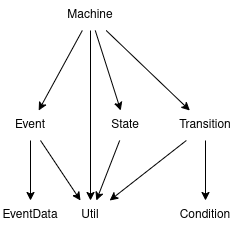
\includegraphics[width=0.7\textwidth]{hierarchy.png}
  \caption{Use hierarchy among modules}
  \label{FigUH}
\end{figure}

\color{black}
%\section*{References}

\bibliographystyle {plainnat}
\bibliography {MG}

\end{document}
